\chapter{Experiment equivalence and algorithms} \label{ch:expeq}

\TODO{Spravit text}.
During the analysis of code-breaking games,
  we repeatedly need to select the next experiment.
When we analyse a strategy, we must prepare a list of experiments
  for the strategy to choose from and
  during the optimal strategy synthesis,
  we need to try all possible experiments, finish the game with the gained knowledge,
  and then select the optimal one.

The set of all experiments is typically very large and not all experiments
  have to be considered.
For example, in the counterfeit-coin problem (\ref{prob-coins}),
  there is a parametrized experiment of weighting 4 coins against 4 coins,
  which has $\frac{1}{2}\cdot {12 \choose 4}\cdot{8 \choose 4} = 17325$
 possible parametrizations.
However, in the initial state
  (i.e. with no knowledge except for the initial constraint),
  all of them are equivalent -- they give us
  the same information regardless of symmetries.

\section{Experiment equivalence}

In this section, we formally define equivalence of two experiments
 and show that we can neglect all but one experiment in each equivalence class.

\begin{definition}[Symmetric experiment]
For an experiment $\exp = (\expt, \param)$ and a permutation $\perm\in\Perm_\Var$,
  a $\perm$-symmetric experiment $\exp^\perm = (\expt, \param')\in\Exp$
  is an experiment of the same type such that
  $\{\form^\perm \in\outcome(\exp)\} = \{\form\in\outcome(\exp^\perm)\}$.
Clearly, no such experiment may exists.
\end{definition}

\begin{definition}[Symmetry group]
We define a \emph{symmetry group} $\symg$ as
  the maximal subset of $\Perm_\Var$ such that for
  every $\perm\in\symg$ and for every experiment $\exp\in\Exp$,
  there exists a $\perm$-symmetric experiment $\exp^\perm$.
\end{definition}

\begin{definition}[Experiment equivalence] \label{def:expeq}
An experiment $\exp_1\in\Exp$ is equivalent to $\exp_2\in\Exp$ with respect to $\form$,
  written $\exp_1\expeq{\form}\exp_2$,
  if and only if there exists a permutation $\perm\in\symg$ such that
 $ \{ \form\wedge\formx \| \formx\in\outcome(\exp_1) \} \equiv
   \{ (\form\wedge\formx)^\perm \| \formx\in\outcome(\exp_2) \} $.
\end{definition}

\begin{example}
Recall the running example from previous chapter, introduced in \autoref{ex:cc-run1}.

Experiment 23 is a $(x_1x_3)$-symmetric experiment of 12, as ($\perm = (x_1x_3)$)
\[
\{ ((x_1 \wedge \neg y) \vee (x_2\wedge y))^\perm,
   ((x_1 \wedge y) \vee (x_2\wedge\neg y))^\perm,
   (\neg (x_1  \vee x_2))^\perm \} =
\{ (x_2 \wedge \neg y) \vee (x_2\wedge y),
   (x_2 \wedge y) \vee (x_2\wedge\neg y),
   \neg (x_2 \vee x_2) \}.
\]

In fact, for each experiment and every permutation $\perm$ stabilizing $y$,
  we can permute the parameters accordingly and get a $\perm$-symmetric experiment.
Therefore, $\symg = \{\perm\in\Perm_\Var \| \perm(y) = y\}$.

Since $\symg$ is also the symmetry group of $\init$, the quotient set of $E$
   by $\expeq{\init}$ has only two equivalence classes --
   weighings of one coin against one and of two coins against two.
For a more complex example, let $\form = \init\wedge\neg(x_1\vee x_2)$.
Experiment $3124$ is now equivalent to $43$ even though the corresponding formulas
  are syntactically different.
\end{example}

\section{Algorithm for experiment equivalence}

In the rest of the section, we suggest an algorithm that decides
  whether two given experiments are equivalent with respect to a given formula.

First, we show a construction of a \emph{base graph}, a graph automorphisms of which are a subset of
  symmetry group $\symg$.
Then we describe construction of a \emph{experiment graph}, which is build on top of the base graph, and prove
  that if graphs of two experiments are isomorphic, the experiments are equivalent.

\subsection{Base graph construction}
Base graph of a game $\game = (\Var, \init, \Sigma, F, \Expt)$ is a coloured graph $B = (V,E,c)$, where
\begin{itemize}
\item $V = \Var \cupdot F$,
\item $(f, x) \in E$ if $f\in F$, $x\in\Var$ and there is a symbol $a\in\Sigma$ such that $f(a) = x$,
\item $(x_1, x_2) \in E$ if $x_1,x_2\in\Var$, there is a symbol $a\in\Sigma$ and two mappings
  $f_1,f_2\in F$ such that $f_1(a) = x_1$, $f_2(a) = x_2$, and
  the mappings appear in the outcomes of an experiment with the same parameter, i.e.
  there is a parametrized experiment $t\in T$ and a number $k <= n_t$ such that
  both $f_1(\$k)$ and $f_2(\$k)$ appear in the outcome formulas of $t$.
\item
  vertices corresponding to the mappings have their own colour, i.e. $c(f) = c_f$
  variables corresponding to variables have one colour $c_{var}$,
  expect for variables that appear directly in some outcome formula of an experiment.
\end{itemize}

\begin{example} \label{ex:cc-runbase}
Base graph for the counterfeit coin problem with 4 coins is shown in
\autoref{fig:base-graph} on the left.
Note that vertices $y$ and $f_x$ have separate labels while
  other vertices are labelled ``variable''.

A more complicated example is the base graph of Mastermind with 3 pegs and 3 colours,
  shown on the right-hand side.
Vertices $f_1, f_2, f_3$ have separate labels, all other vertices are labelled ``variable''.
For simplicity, we leave out symbol $x$ in the figure, e.g.
  write $1A$ instead of $x_{1A}$.\eqed
\begin{figure}[h]
\begin{center}
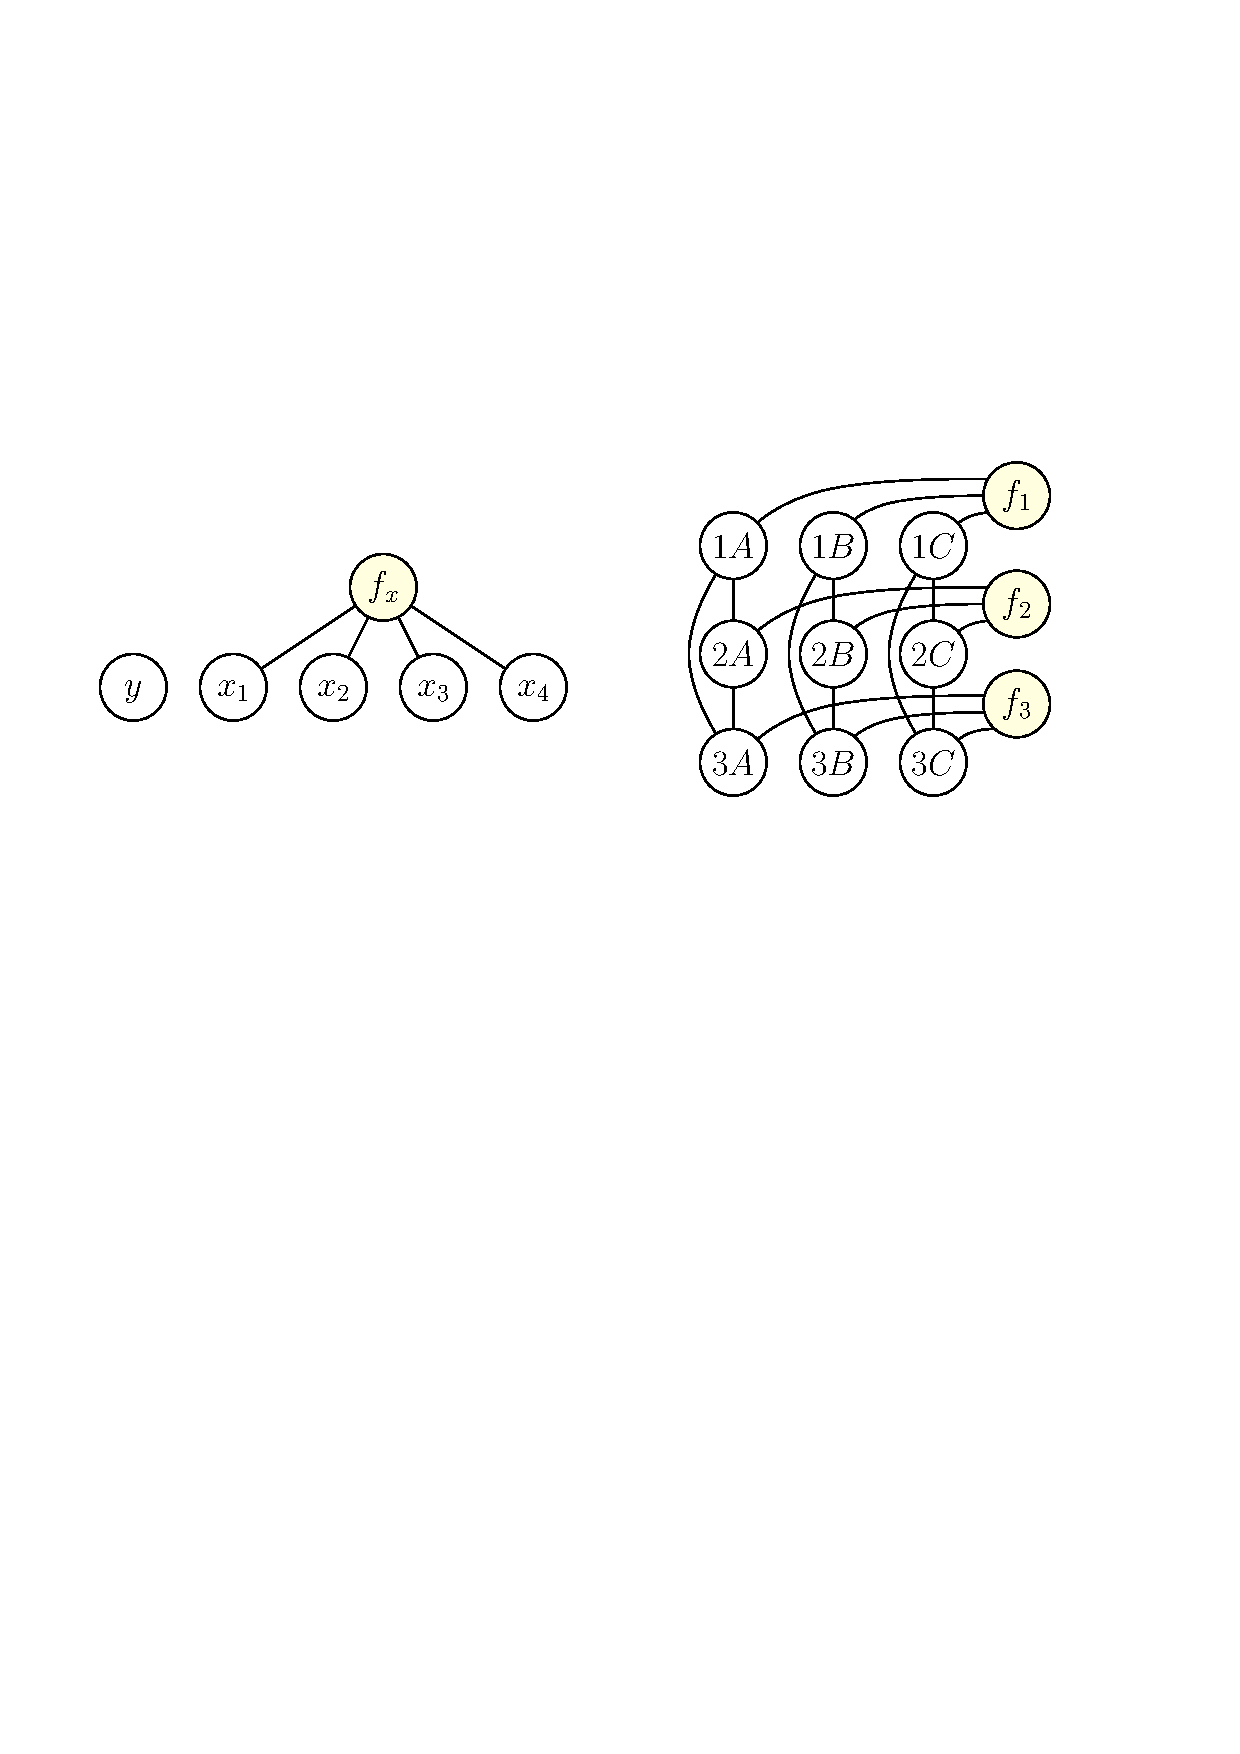
\includegraphics[width=.7\textwidth]{pictures/base-graph.pdf}
\caption{Base graph for the counterfeit coin problem with 4 coins (left) and\\
  for Mastermind with 3 pegs and 3 colours (right).}
\label{fig:base-graph}
\end{center}
\end{figure}
\end{example}

\begin{lemma}
Let  $\perm$ be an automorphism of $B$. Then $\perm|_\Var \in\symg$.
\end{lemma}

\begin{proof}
Blah. \qed
\end{proof}

\subsection{Experiment graph}

Let $\form\in\Form_X$.
A \emph{tree of $\form$ rooted with label $l$}
  is a graph created from the syntax tree of $\form$
  by unification of leaves that correspond to the same variable.
The vertices of the graph are labelled by their type (e.g. ``variable'', ``and-operator'', etc.)
and one special node with label $l$ is added and connected to the root of the syntax tree,
  i.e. to the top-level operator of $\form$.

Let $B$ be a base graph of the game, $\form\in\Formr$ some partial knowledge
  and $e$ an experiment.
The experiment graph $B_{\form, e}$ is constructed as follows:
\begin{itemize}
\item Start with $B$.
\item Add a tree of $\form$ rooted with label ``knowledge''.
\item For each outcome $\formx\in\outcome(e)$, add a tree of $\formx$ rooted with label ``outcome''.
\end{itemize}

\begin{theorem}
If $B_{\form, e_1}$ is isomorphic to $B_{\form, e_2}$, then
 $e_1 \expeq{\form} e_2$.
\end{theorem}

\begin{proof}
Blah. \qed
\end{proof}

\begin{example}
Recall the running example of the counterfeit coin problem with 4 coins.
Base graph for the game was shown in \autoref{ex:cc-runbase}.
Let $\form=\init\wedge\neg(x_1\vee x_2)$ (knowledge after the experiment 12
  that resulted in ``='' outcome) and $e$ is experiment $3124$.
Experiment graph $B_{\form, e}$ is shown in \autoref{fig:exp-graph},
  Ex$_1$ denotes the $\exactlyk{1}$ operator.
\begin{figure}[h]
\begin{center}
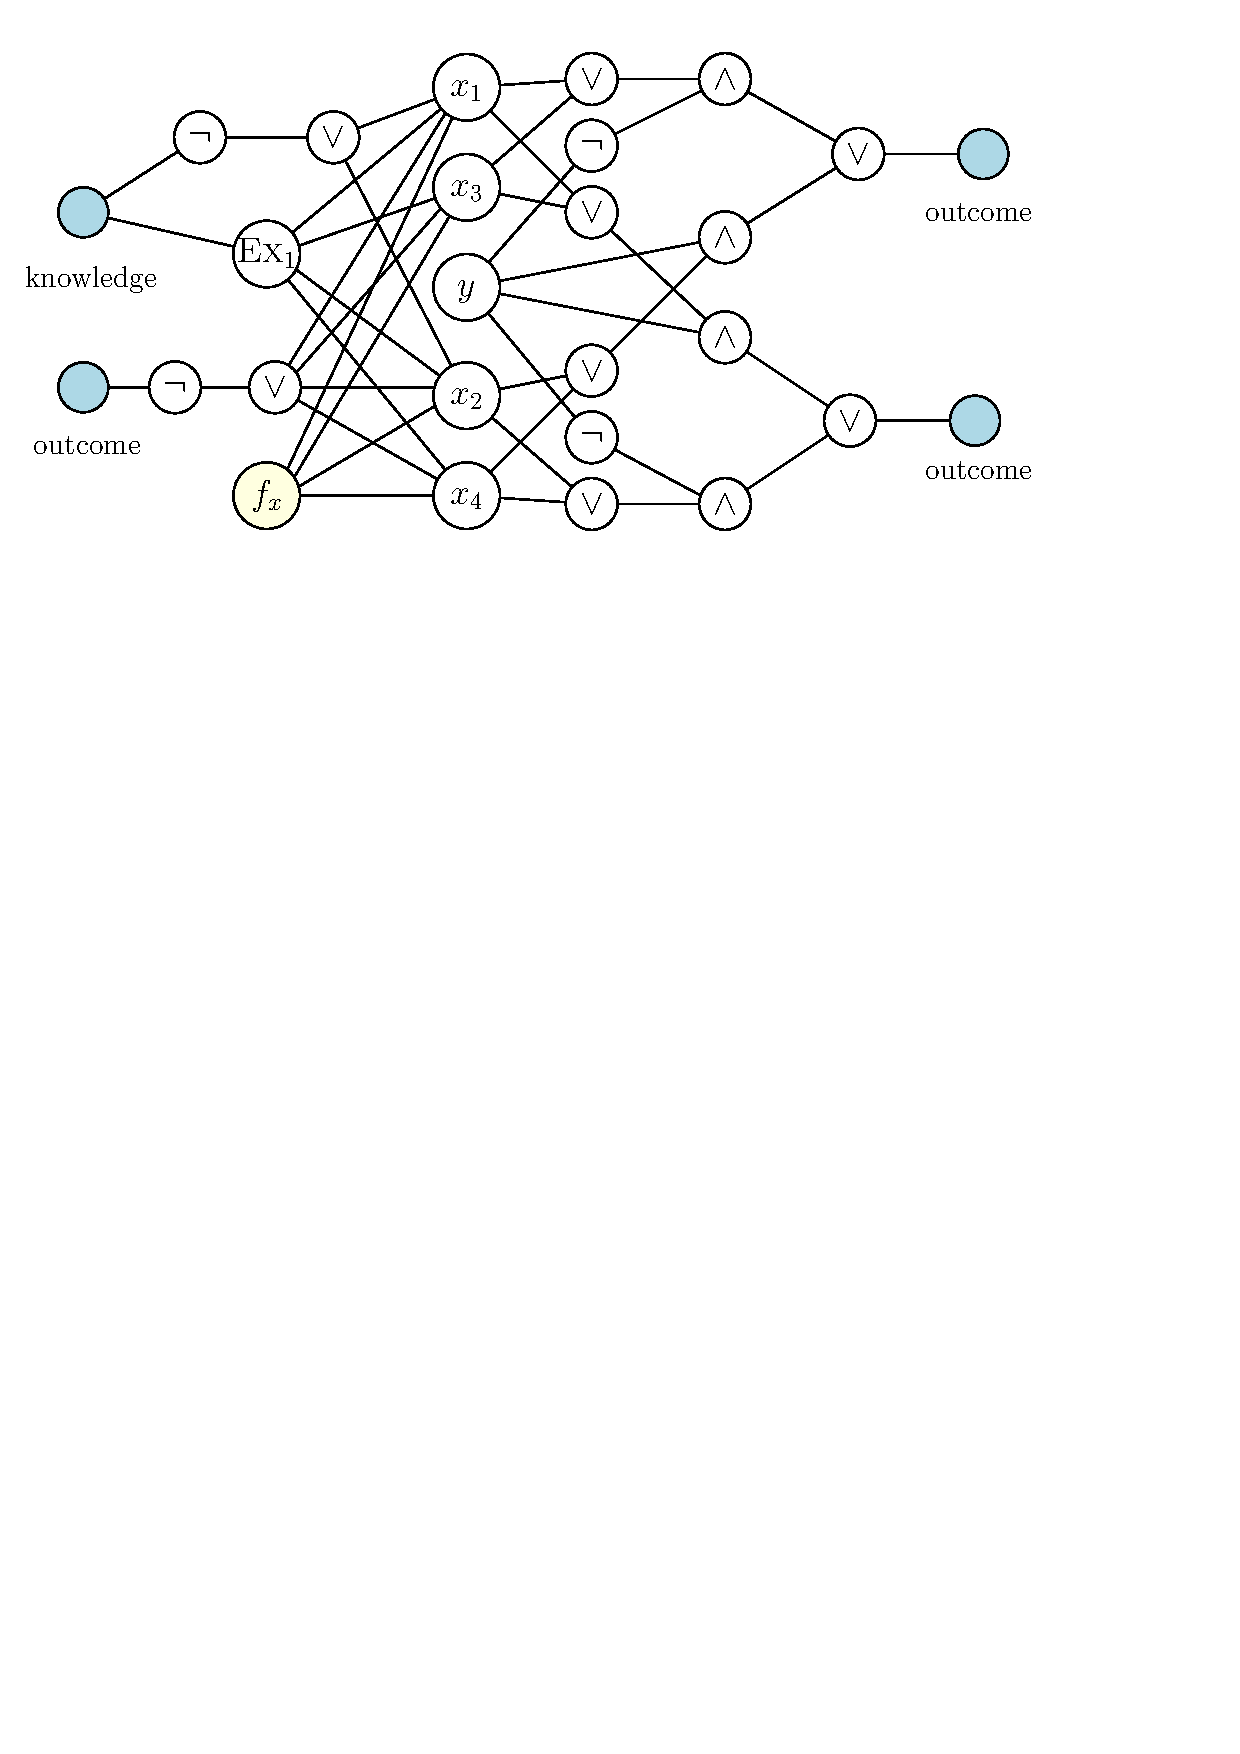
\includegraphics[width=.7\textwidth]{pictures/exp-graph.pdf}
\caption{Experiment graph for 3124 with knowledge $\init\wedge\neg(x_1\vee x_2)$.}
\label{fig:exp-graph}
\end{center}
\end{figure}

Unfortunately, the graph for experiment 43 is clearly not isomorphic to this graph,
although the experiments are equivalent with respect to $\form$.
We address this problem in the following.
\end{example}

\subsection{Improvement by fixed variables}

The previous example shows that the formulated method, as explained above,
  does not detect some basic equivalences.
To address the problem, we suggest the following improvement to the construction
  of $B_{\form, e}$.
\begin{enumerate}
\item Compute fixed variables of formula $\form$.
\item Simplify formula $\form$ with the knowledge of fixed variable.
\item Simplify the outcomes of $e$, formulas $\formx\in\outcome(e)$, with
  the knowledge of fixed variables in $\form$.
\item Construct the graph as described above.
\item Label the vertices corresponding to fixed variables with ``false'' or ``true''
  according to their fixed value.
\end{enumerate}

\begin{example}
Let us apply the suggested improvement on the previous example.
\autoref{fig:exp-graph-sim} shows the experiment graph $B_{\form, e}$
  constructed after the simplification with the knowledge of fixed variables.
Compare the structure with the graph in \autoref{fig:exp-graph}.

\begin{figure}[h]
\begin{center}
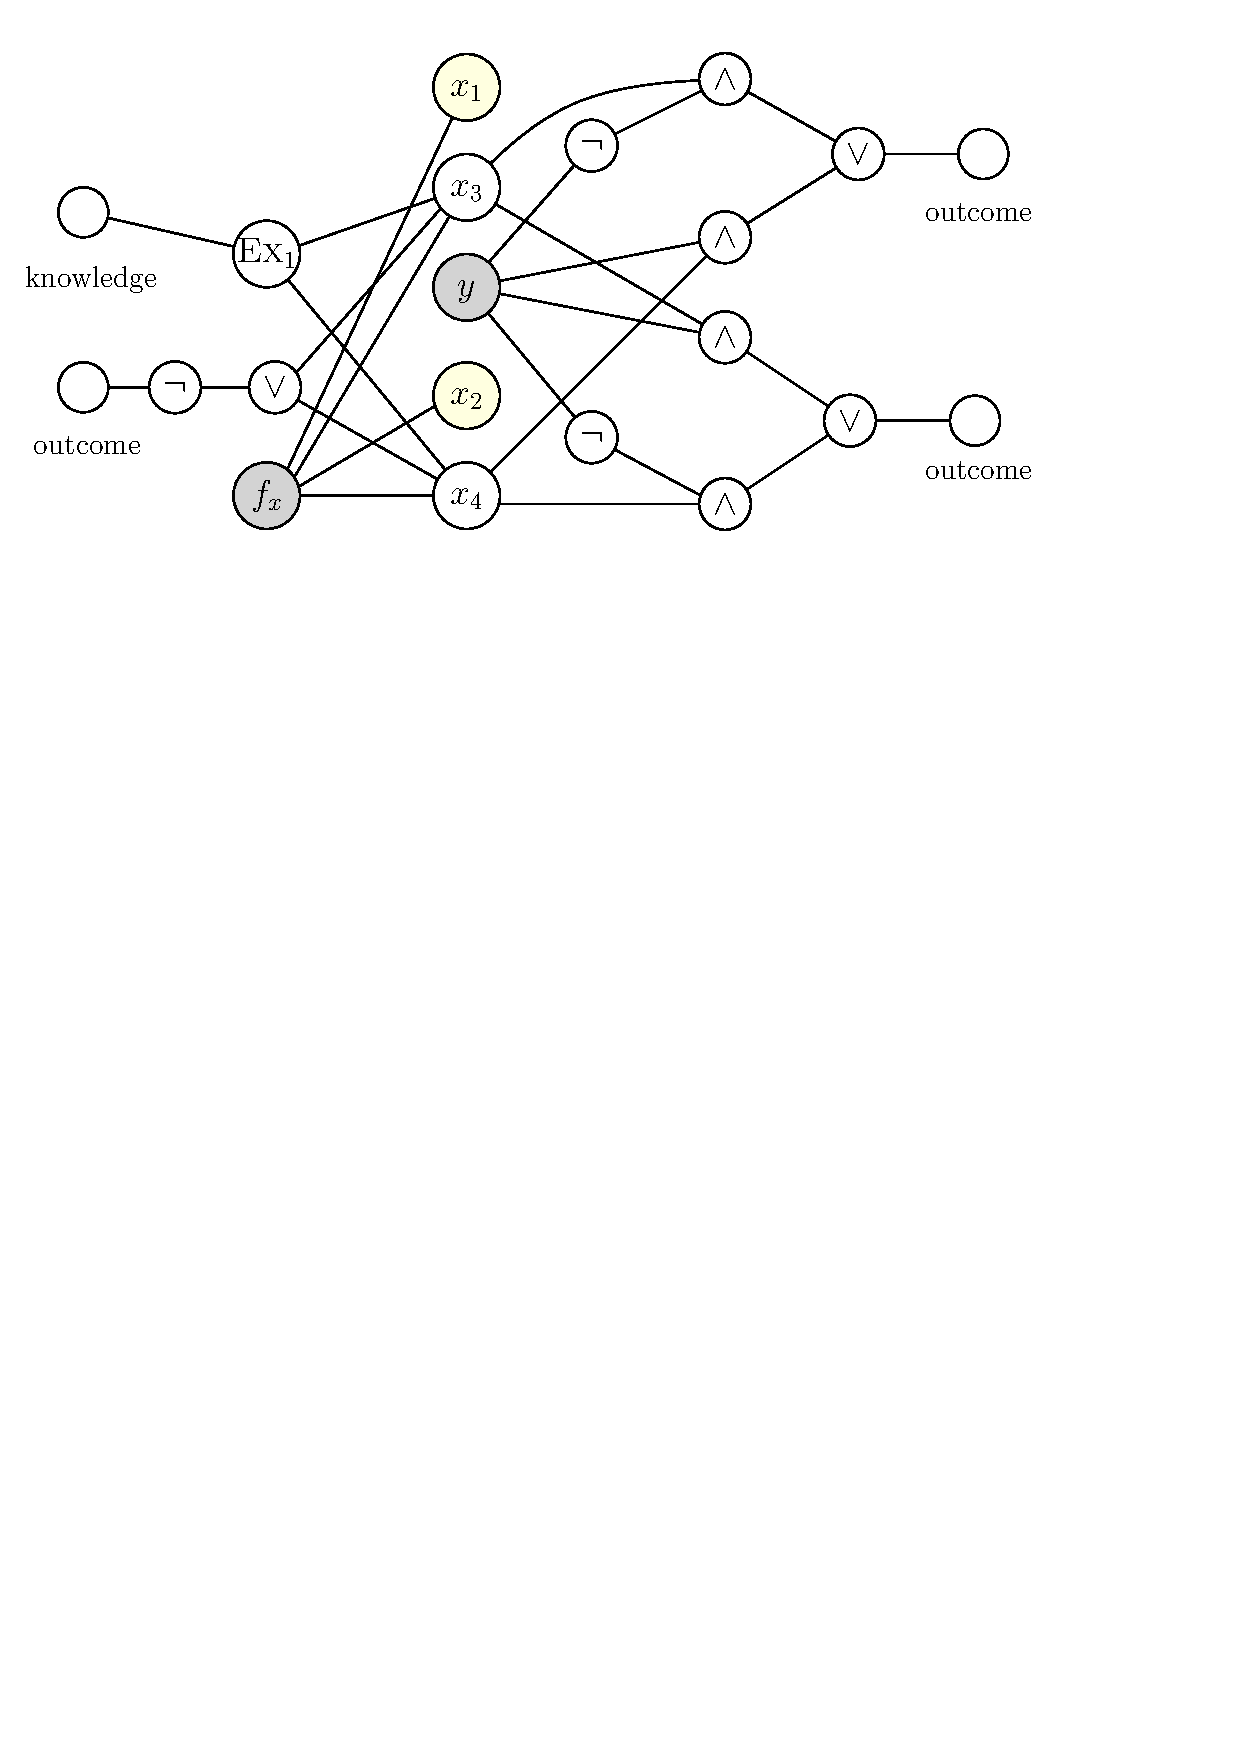
\includegraphics[width=.7\textwidth]{pictures/exp-graph-sim.pdf}
\caption{Simplified experiment graph for 3124 with knowledge $\init\wedge\neg(x_1\vee x_2)$.}
\label{fig:exp-graph-sim}
\end{center}
\end{figure}
Now, vertices $x_1$ and $x_2$ are labelled ``false'' and are connected
  only to vertex $f_x$.
The graph is now isomorphic to the graph of experiment $43$.\eqed
\end{example}

The algorithm for generation of non-equivalent experiments with respect to a formula $\form$
  is now a straightforward application of the method described in this section.
Details are described in \autoref{alg:noneqexp}.

\begin{algorithm}[h!]
\caption{Generation of non-equivalent experiments with respect to~$\form$}
\label{alg:noneqexp}
\DontPrintSemicolon
$B <- $ contruct the base graph for the game\;
$fixed <- $ compute the fixed variables of $\form$\;
$\form' <- $ substitude values for $fixed$ in $\form$ and simplify\;
colour nodes in $B$ corresponding to fixed variables with special colors (special color for true, special color for false)\;
$B <- B$ joined with graph for formula $\form'$ rooted with a node of special color ``knowledge''\;
$S <- \emptyset$\;
$hash <- $ an empty hash table for graphs\;
\For{$e\in E$}{
  $B_e <- $ clone $B$\;
  \For{$\formx\in\outcome(e)$} {
    $\formx' <- $ substitude values for $fixed$ in $\formx$ and simplify\;
    $B_e <- B_e $ joined with graph for formula $\formx'$ rooted with a node of special color ``outcome''\;
  }
  $B_e <- $ canonize $B_e$\;
  \If{$B_e$ is not present in $hash$}{
    $hash$.insert($B_e$)\;
    $S <- S \cup \{e\}$\;
  }
}
\Return{$S$}
\end{algorithm}


\section{Well-formed check}

Experiment equivalence can be used in the verification
  of the well-formed property of a game.

\begin{lemma} \label{lma:well-formed}
  Let $S\subseteq E$ be a subset of experiments
  such that for every $e\in E$, there exists $e'\in S$
   such that $e\expeq{\init}e'$.
  If the formula $\init ==> \exactlyk{1}(\outcome(e'))$ is a tautology for
  all $e'\in S$, then the game is well-formed.
\end{lemma}

\begin{proof}
To get a contradiction, suppose the game is not well formed, i.e.
  there is $e\in E$ and $v \in \Vals$ such that the number of
  formulas in $\outcome(e)$ satisfied by $v$ is not equal one.

If $e\in S$, the formula $\init ==> \exactlyk{1}(\outcome(e'))$ is not
  satisfied by $v$. Contradiction.

Otherwise, there exists $e'\in S$ such that $e\expeq{\init}e'$, i.e.
  there exists $\perm\in\Perm_\Var$ such that
$\{ \init\wedge\formx \| \formx\in\outcome(e) \} =
 \{ (\init\wedge\formx)^\perm \| \formx\in\outcome(e') \}$.
Since $\init ==> \exactlyk{1}(\outcome(e'))$ is a tautology,
  the permuted formula
  $\init^\perm ==> \exactlyk{1}(\formx^\perm \| \formx\in\outcome(e'))$
  is a tautology as well.
Therefore, exactly one formula from the set
 $ \{ (\init\wedge\formx)^\perm \| \formx\in\outcome(e') \}$
 is satisfiable and the same holds for
  $\{ \init\wedge\formx \| \formx\in\outcome(e) \}$,
 which implies that
 $\init ==> \exactlyk{1}(\outcome(e))$
 is a tautology. \qed
\end{proof}


\section{Strategy analysis}

The following theorem gives us a right to disregard equivalent experiments
  during analysis of a one-step look-ahead strategies.

\begin{theorem}
Let $f: 2^\Formr ->\Rset$ be a function such that
$f(\formset) = f(\{\form^\pi \| \form\in\formset\})$ for any permutation
$\pi\in\Perm_\Var$. Let $<$ be a total order of experiments $E$.
Let $\stg$ be a one-step look-ahead strategy with respect to $f$ and $<$, and
let $\form$ be a formula.
Suppose there are experiment $e_1$, $e_2$ such that $e_1\expeq{\form}e_2$ and $e_1<=e_2$.
Then $\stg(\form) \not= e_2$.
\end{theorem}

\begin{proof}
If follows directly from \autoref{def:expeq} and the property of $f$ that
$f(\{\form\wedge\formx\| \formx\in\outcome(e_1)\}) =
 f(\{\form\wedge\formx\| \formx\in\outcome(e_2)\})$.
Since $e_1 < e_2$, the strategy always prefers $e_1$ to $e_2$. \qed
\end{proof}

\begin{algorithm}[h]
\caption{Strategy analysis of one-step look-ahead with respect to $f$}
\label{alg:stganalysis}
\DontPrintSemicolon
$globalsum <- 0$\;
$globalmax <- 0$\;
\textsc{Analyze}($\init$, 1)\;
\Return$ (global-max,\; global-sum \;/\; \numval\init)$\\\hrulefill\;
\SetKwProg{optfun}{Function}{}{}
\optfun{\textsc{Analyse}\textnormal{($\form$, $depth$)}}{
$choice <- $None\;
$bestvalue <- \infty$\;
\For{$e\in E$(variant 1) or $e\in$\textsc{Non-Equiv-Experiments($\form$)} (variant 2)}{
  $value <- f(e)$
  \If{$value < bestvalue$} {
    $choice <- e$\;
    $bestvalue <- value$\;
  }
}
\For{$\formx\in\outcome(e)$}{
  \lIf{not $\SAT{\form\wedge\formx}$}{continue}
  \eIf{$\numval(\form\wedge\formx) == 1$}{
    $globalsum <- globalsum + depth$\;
    $globalmax <- max(globalmax, depth)$\;
  }{
    \textsc{Analyse}($\form\wedge\formx$, $depth + 1$)\;
  }
}
}{}
\end{algorithm}

\section{Optimal strategy synthesis}

Backtracking is the basic method for worst-case and average-case
  optimal strategy synthesis.
Our goal in this section is to prove that we can disregard
  equivalent experiments and thus significantly
  reduce branching of the algorithm in every step.

\newcommand{\optval}{\kappa}
\newcommand{\optexp}{\varepsilon}
\newcommand{\optvale}{\kappa_\textrm{exp}}
\newcommand{\optexpe}{\varepsilon_\textrm{exp}}

First, let us define $\optval(\form)$ and $\optvale(\form)$ as
 the optimal number of experiments needed to reveal the secret code
  when starting with knowledge $\form$
  in the worst-case and in the average-case, respectively.
We can say that $\optval(\form)$, resp. $\optvale(\form)$ is
  the worst-case, resp. average-case number of experiments of
  a worst-case, resp. average-case optimal strategy
  if we change the initial constraint of the game to $\form$.

Similarly, we define $\optval(\form, e)$ and $\optvale(\form, e)$ as
  the optimal number of experiment needed to reveal the secret code
  when starting with knowledge $\form$ and
  with $e$ as the first experiment.

There is an obvious relationship between $\optval(\form)$ and $\optval(\form,e)$
  and between $\optvale(\form)$ and $\optvale(\form,e)$.
For any $\form\in\Formr$,
\begin{equation}
\optval(\form) = \min_{e\in\Exp}\optval(\form, e),\textrm{ and }
\hspace{1cm}
\optvale(\form) = \min_{e\in\Exp}\optvale(\form, e).
\label{opttriv}
\end{equation}

Further, we can compute $\optval(\form, e)$ and $\optvale(\form, e)$
  from the optimal values for the subproblems after one experiment.
These relationships are based on the definitions of the worst-case
  and average-case number of experiments of a strategy
  ($\lenmax{\stg}$ and $\lenexp{\stg}$).
For any $\form\in\Formr$ and $e\in E$,
\begin{align}
\optval(\form, e) &= \left\{\begin{array}{ll}
 0 & \textrm{ if }\numval{\form} = 1, \\
 \infty & \textrm{ if }\exists\formx\in\outcome(e).\; \form\wedge\formx\equiv\form, \\
 1 + \max_{\formx\in\outcome(e)}\optval(\form\wedge\formx) &
 \textrm{ otherwise. }
\end{array}\right.\label{optval}\\
\optvale(\form, e) &= \left\{\begin{array}{ll}
 0 & \textrm{ if }\numval{\form} = 1, \\
 \infty & \textrm{ if }\exists\formx\in\outcome(e).\; \form\wedge\formx\equiv\form, \\
 1 + \frac{\sum_{\formx\in\outcome(e)}\numval{(\form\wedge\formx)}\cdot\optvale(\form\wedge\formx)}{\numval{\form}} &
 \textrm{ otherwise. }
\end{array}\right.\label{optvale}\\
\end{align}

Let us now define a set of optimal choices in a state.
For a $\form\in\Formr$, we define
\begin{align*}
\optexp(\form) &= \{ e\in E \| \forall e'\in E.\; \optval(\form, e) <= \optval(\form, e') \},\textrm{ and }\\
\optexpe(\form) &= \{ e\in E \| \forall e'\in E.\; \optvale(\form, e) <= \optvale(\form, e') \}.
\end{align*}

The following lemma is a straightforward consequence of the definitions of $\optval$ and~$\optexp$.

\begin{lemma}
Let $\stg$ be a strategy such that $\stg(\form)\in\optexp(\form)$ for every $\form\in\Formr$.
Then $\stg$ is worst-case optimal.
Similarly, let $\stg'$ be a strategy such that $\stg'(\form)\in\optexpe(\form)$ for every $\form\in\Formr$.
Then $\stg'$ is average-case optimal.
\end{lemma}

Now we are ready for the main theorem, which gives as a right to consider
  only one experiment from
  each equivalence class of $E/\expeq{\form}$
  in the state where the
  accumulated knowledge is $\form$.
The exact algorithm for optimal strategy synthesis
  with further optimizations is described in \autoref{s:cobra-modes}.

\begin{theorem}
For every $\form\in\Formr$,
\begin{enumerate}
\item $\optval(\form) = \optval(\form^\perm)$ and $\optvale(\form) = \optvale(\form^\perm)$ for all $\perm\in\symg$, and
\item if $e_1\expeq{\form} e_2$, then $e_1\in\optexp(\form) \Leftrightarrow e_2\in\optexp(\form)$ and
  $e_1\in\optexpe(\form) \Leftrightarrow e_2\in\optexpe(\form)$.
\end{enumerate}
\end{theorem}

\begin{proof}
The proof for the worst case ($\optval, \optexp$)
  and for the average-case ($\optvale, \optexpe$) is exactly the same,
  so we prove it only for worst-case.

Since $\perm\in\symg$, there exists a $\perm$-symmetric experiment $e^\perm$
  for every $e\in E$.
Recall that $\outcome(e^\perm) = \{ \formx^\perm \| \formx\in\outcome(e)\}$.
We show by induction on the number of models of $\form$
  that $\optval(\form, \exp) = \optval(\form^\perm, \exp^\perm)$,
  which is sufficient for the first part.

As $\numval{\form} = \numval{\form^\perm}$, the statements follows directly from
  (\refeq{opttriv}) and (\refeq{optval}) for formulas with one model.
For the induction step, observe that
  $\numval(\form^\perm \wedge \formx^\perm) = \numval(\form\wedge\formx)$
  and
  $\optval(\form^\perm \wedge \formx^\perm) = \optval(\form\wedge\formx)$
  if $\form \not\equiv \form\wedge\formx$, by the induction hypothesis.
The statement now follows from (\refeq{optval})
  as the right sides are equal.

For the second part, it suffices to prove that
  $\optval(\form, e_1) = \optval(\form, e_2)$.
As the experiments are equivalent, there exists a permutation $\perm\in\symg$,
 such that
 $\{\form\wedge\formx \|\formx\in\outcome(e_1)\} =
 \{(\form\wedge\formx)^\perm \|\formx\in\outcome(e_2)\}$.
The equation now follows from (\refeq{optval}) and the facts that
 $\numval\form=\numval\form^\perm$ and $\optval(\form) = \optval(\form^\perm)$
 (proven in the first part). \qed
\end{proof}

A recursive algorithm for the computation of the value
  of an average-case optimal strategy,
  $\optvale(\form)$ is shown in \autoref{alg:acopt}.
The algorithm is based on equation (\refeq{optvale}) and
  the previous theorem.

Apart from formula $\form$, the recursive function takes another argument, $opt$,
  which is used for branch pruning.
The value of $opt$ is the best value of $\optvale(\form, e)$
  that was found so far.
Clearly, if we can be sure that $\optvale(\form, e') > opt$, we are not interested
  in the exact value as the experiment will not be selected anyway.
A lower bound on $\optvale(\form, e')$ can be computed using \autoref{lma:lbound}.

The inital value of $opt$ should be $\infty$ or an upper bound on $\optvale(\init, e)$.


\begin{algorithm}[h]
\caption{Synthesis of average-case optimal strategy.}
\label{alg:acopt}
\DontPrintSemicolon
\SetKwProg{optfun}{Function}{}{}
\optfun{\textsc{Optimum}\textnormal{($\form$, $opt$)}}{
\lIf{$\numval{\form} = 1$}{\Return{0}}
$ lb <- \textsc{LowerBound}(\form)$\;
\lIf{$lb > opt$}{\Return{$\infty$}}
compute subset of experiments $S$ such that
  $e\in E ==> \exists e'\in S.\;e\expeq{\form}e'$\;
% $ b <- $ maximal number of satisfiable outcomes of an experiment in $S$\;
% $ lb <- \textsc{LowerBound}(\form, b)$\;
% \lIf{$lb > opt$}{\Return{$\infty$}}
\For{$s\in S$, ordered by $\max_{\formx\in\outcome(s)}\numval(\form\wedge\formx)$}
{
  \lIf{only one of $\form\wedge\formx$, $\formx\in\outcome(s)$ is satisfiable}{continue}
  $ val <- 0 $\;
  \For{$\formx\in\outcome(s)$} {
    \lIf{$\SAT{\form\wedge\formx}$}{
    $~\;\;\;\;\;val <- val + \numval(\form\wedge\formx)\cdot
      (1 + \textsc{Optimum}(\form\wedge\formx,\; opt))$}
  }
  $val <- val \;/\; \numval(\form)$\;
  \lIf{$val < opt$}{$opt <- val$}
}
\Return{$opt$}
}{}
\end{algorithm}

Note that the order of experiments on line 7
  is not necessary for correctness of the algorithm.
Our goal is to find a good experiment as soon as possible,
  because this allows us to prune many branches in the beginning.


% \begin{definition}[Consistent strategy]
% A memory-less strategy $\stg$ is \emph{consistent} if and only if
%   for every $\form\in\Form_\Var$ and every $\perm\in\symg$, there
%   exists $\permx\in\symg$ such that $\form^\perm \equiv \form^\permx$ and
%   $\stg(\form^\permx) = \stg(\form)^\permx$.
% \end{definition}

% \TODO{Example, na kterém bude vidět, že jednoduchá definice nevyhovuje, protože můžu vzít symetrie $\form$ a dostanu, že to má dávat různé věci.}

% \begin{lemma}
% Let $\stg$ be a memory-less strategy.
% There exists a consistent memory-less strategy $\stgx$ such that
%   $\stglen{\stg}{\val} >= \stglen{\stgx}{\val}$
%   for all $\val\in\Val_X$ satisfying $\init$.
% \end{lemma}

% \begin{proof}
% Similar to the proof of Lemma \ref{lma-opt-memoryless}.
% Let us choose any total order $\form_1, \form_2, ...$ of $\Form_\Var$ such that
% if $\form_i$ implies $\form_j$, then $i <= j$.
% We build a sequence of strategies $\stg_0, \stg_1, \stg_2, ...$ in the following way:
% Let $\stg_0 = \stg$ and for $i > 0,$
% \begin{equation}
% \stg_i(\form) = \left\{
%  \begin{array}{lll}
%  \stg_{i-1}(\form) & \textrm{ if } \not\exists\perm\in\symg.\form^\perm\equiv\form_i \\
%  \procstg{\stg_{i-1}}{\val_i}(k_i + 1) &
%     \textrm{ if } \exists\perm\in\symg.\form^\perm\equiv\form_i\textrm{, where }
%     (v_i, k_i) = \argmin_K \stglen{\stg_{i-1}}{v} - k,\\
%     & \textrm{ and }
%     K = \{(v, k)\in\Val\times\Nseto \| \exists\perm.\stgknow{\stg_{i-1}}{v}{k}^\perm\equiv\form_i\}.
%     \vspace{-2.5ex}
%  \end{array}
%  \right.
%  \vspace{2.5ex}
% \end{equation}
% We prove that $\stglen{\stg_{i}}{v} <= \stglen{\stg_{i-1}}{v}$.
% If there is no $k$ and $\perm$ such that $\stgknow{\stg_i}{v}{k}^\perm\equiv\form_i$ then
%   the processes $\procstg{\stg_i}{v}$ and $\procstg{\stg_{i-1}}{v}$ are the same.
% If the is such $k$ and \TODO{...}.

% The last strategy of the sequence is consistent and satisfies the
%   condition in the lemma. \qed
% \end{proof}

% \begin{theorem}
% Let $\stg, \stgx$ be two consistent memory-less strategies, such that
% $\stg(\form) \expeq{\form} \stgx(\form)$ for any $\form\in\Form_\Var$.
% There is a bijection $f:\Val_\Var -> \Val_\Var$ such that
% $\stglen{\stg}{\val} = \stglen{\stgx}{f(\val)}$.
% \end{theorem}

% \begin{proof}
% First, we prove by induction for any $k\in\Nseto$,
%   there is a permutation $\perm\in \symg$ such that
%   $(\stgknow{\stg}{\val}{i})^\perm = \stgknow{\stgx}{\val^\perm}{i}$
%   for all $i\in\Nseto$, $i<=k$.
% For better readability, let
%   $\know_k = \stgknow{\stg}{\val}{k}$ and
%   $\knowx_{k, \perm} = \stgknow{\stgx}{\val^\perm}{k}$

% For $k=0$, take $\perm = \idperm_\Var$.
% Clearly, $\stgknow{\stg}{\val}{0} = \init = \stgknow{\stgx}{\val^\idperm}{0}$.

% For the induction step, suppose we have $\perm\in\symg$ such that
%   $\know_i^\perm = \knowx_{i, \perm}$ for $i <= k$.
% Further, suppose $\perm$ is such that
%   $\stg(\know_k^\perm) = \stg(\know_k)^\perm$. \TODO{Víc zdůvodnit.}

% Let $e_1 = \stg(\know_k)$, $e_2 = \stgx(\knowx_{k, \perm})$
%   be the $(k+1)$-th experiments  of the strategies.
% It holds
% \begin{equation}
% e_2 = \stgx(\knowx_{k, \perm})
%     \expeq{\knowx_{k, \perm}}  \stg(\knowx_{k, \perm})
%     \stackrel{IH}{=} \stg(\know_k^\perm)
%     = \stg(\know_k)^\perm
%     = e_1^\perm \label{eq:expsym}\tag{$\sim$}
% \end{equation}

% and, therefore, there exists $\permx\in\symg$ such that
% \begin{align}
%  \{ \knowx_{k, \perm} \wedge \formx \| \formx\in\outcome(\exp_2) \} &= %\stackrel{(\refeq{eq:expsym})}{=}
%  \{ (\knowx_{k, \perm} \wedge \formx)^\permx \| \formx\in\outcome(\exp_1^\perm) \} = \label{eq:sets}\tag{*}\\
% &= \{ (\know_k^\perm \wedge \formx^\perm)^\permx \| \formx\in\outcome(\exp_1) \} =
%  \{ (\know_k \wedge \formx)^{\permx\perm} \| \formx\in\outcome(\exp_1) \}
% \end{align}
% As $\permx\in\symg$ and $\symg$ is a permutation group, $\permx\perm\in\symg$.

% Since the game is well-formed,
%   $v$ satisfies exactly one formula in
%   $\{ \know_k \wedge \formx \| \formx\in\outcome(\exp_1) \}$.
% Therefore $v^{\permx\perm}$ satisfies exactly one formula
%   in
%   $\{ (\know_k \wedge \formx)^{\permx\perm} \| \formx\in\outcome(\exp_1) \}  =
%    \{ \knowx_{k, \perm} \wedge \formx \| \formx\in\outcome(\exp_2) \}$,
%   which means that $v^{\permx\perm}$ satisfies $\knowx_{k, \perm}$.
% \TODO{Tohle nefugujeee!}
% From Lemma \ref{lma-accruedknowledge},
%   $\knowx_{k, \perm} = \knowx_{k, \permx\perm}$.
% Both $\know_{k+1}^{\permx\perm}$ and $\knowx_{k+1, \permx\perm}$ is thus the only
%   formula from (\refeq{eq:sets}) satisfied by $v^{\permx\perm}$ and, therefore,
%   $\know_{k+1}^{\permx\perm} = \knowx_{k+1, \permx\perm}$.


% Now for a fixed $\val$, take $k = \stglen{\stg}{\val}$, take
%   $\perm\in\symg$ such that
%   $(\stgknow{\stg}{\val}{k})^\perm = \stgknow{\stgx}{\val^\perm}{k}$
%   and define $f(\val) = \val^\perm$.
% Since
%  $(\stgknow{\stg}{\val}{i})^\perm = \stgknow{\stgx}{f(\val)}{i}$
%  for $i <= k$
%  and variable permutation preserves the number of models of a formula, i.e.
%   $\numval{\form} = \numval{\form^\perm}$ for any
%   $\form\in\Form_\Var$, $\perm\in\Perm_\Var$,
%  we have
%   $\stglen{\stg}{\val} = \stglen{\stgx}{f(\val)}$.
% % \TODO{It remains to show that $f$ is a bijection.}
%   % Suppose $f$ is not injective, and $f(\val_1) = f(\val_2)$.
%   % By definition, the only model of
%   \qed
% \end{proof}

% \begin{corollary}
% Let $\stg_1, \stg_2$ be two consistent memory-less strategies, such that
%   $\stg_1(\form) \expeq{\form} \stg_2(\form)$ for any $\form\in\Form_\Var$.
% Then $\lenmax{\stg_1} = \lenmax{\stg_2}$
%   and $\lenexp{\stg_1} = \lenexp{\stg_2}$.
% \end{corollary}

% For any accrued knowledge $\form$, this lemma gives us the right
% to consider only one of the experiments
% $\exp_1, \exp_2$ if $\exp_1 \sim_\form \exp_2$.

% \TODO{algorithm for optimal algorithm synthesis}
